\section{Evaluation}

We evaluate \systemname\ under a 48\,GB single-GPU envelope. The study asks whether dynamic precision residency (1)~recovers quality lost to a fully resident low-precision baseline, (2)~maintains useful latency and throughput as routed activation becomes dense, (3)~benefits from each policy and mechanism component, and (4)~obeys its memory invariant across precision budgets. Static PTQ is the no-migration reference; an executable offloading system is included where its public implementation supports the evaluated checkpoint.

\subsection{Experimental Setup}
\label{sec:eval-setup}

\begin{table}[t]
  \centering
  \caption{Configuration of evaluated MoE models.}
  \label{tab:moe_config}
  \vspace{-0.5em}
  \setlength{\tabcolsep}{4pt}
  \resizebox{\linewidth}{!}{
  \begin{tabular}{lccc}
    \toprule
    & \textbf{Qwen3-30B} & \textbf{Qwen3-Next-80B} & \textbf{Phi-3.5-MoE} \\
    \midrule
    Total Parameters & 30.5B & 80B & 42B \\
    Activated / Token & 3.3B & 3B & 6.6B \\
    Reference Tier & FP16 & INT4 & FP16 \\
    Expert Weight Fraction & 95\% & 96\% & 96\% \\
    Layers & 48 & 48 & 32 \\
    Routed Experts / Layer & 128 & 512 (+1 shared) & 16 \\
    Top-$K$ & 8 & 10 & 2 \\
    \bottomrule
  \end{tabular}}
\end{table}

\noindent\textbf{Models.}
We use \nolinkurl{Qwen/Qwen3-30B-A3B-Instruct-2507}~\cite{qwen3technicalreport}, \nolinkurl{Qwen/Qwen3-Next-80B-A3B-Instruct}~\cite{qwen3nextmodelcard}, and \nolinkurl{microsoft/Phi-3.5-MoE-instruct}~\cite{abdin2024phi3} (\autoref{tab:moe_config}).

\noindent\textbf{Benchmarks.}
WikiText-2~\cite{merity2016pointer} (perplexity), MMLU-Pro~\cite{wang2024mmlu}, GPQA~\cite{rein2024gpqa}, AIME25~\cite{zhang2025aime25}, GSM8K~\cite{cobbe2021gsm8k}, and HumanEval~\cite{chen2021evaluating}.

\noindent\textbf{Evaluation protocol.}
We use the complete pinned test splits of MMLU-Pro and GSM8K, all 198 GPQA-Diamond questions, all 30 AIME25 problems, and all 164 HumanEval tasks. GPQA answer choices are shuffled once with seed 42 and the resulting order is shared by every method. Multiple-choice accuracy uses the conditional log-likelihood of each complete answer label rather than a single token; all labels for one question are scored in one unpadded batch so an online precision switch cannot occur between candidates. Numeric answers are taken from an explicit final-answer field, or from the last generated integer when the field is absent; matching an intermediate number does not count. HumanEval reports pass@1 only after executing the official tests with greedy decoding. WikiText perplexity is computed over at most 128 exact 2,048-token windows, with overlapping context labels masked when a shorter stride is used; each artifact stores every window boundary, effective target-token count, mean loss, and NLL so the aggregate can be independently recomputed. The five-task average is a descriptive effect size, not a pooled significance test. For paired method comparisons, we match sample identifiers and dataset fingerprints, apply an exact McNemar test to each task, and use Holm correction across the five tests.

\noindent\textbf{Hardware and stack.}
All experiments run on a single NVIDIA RTX~A6000 (48\,GB device memory). \systemname\ is integrated into a PyTorch/Transformers-based MoE inference stack~\cite{paszke2019pytorch,wolf2020transformers}. Hot routed experts use a higher-precision tier (FP16 for Qwen3-30B and Phi-3.5-MoE; INT4 for Qwen3-Next-80B); cold routed experts remain at a lower tier (INT4 or INT2, respectively). The Qwen3-Next shared expert remains fixed and is counted with non-routed weights.

\noindent\textbf{Measurement and provenance.}
Quality runs use greedy decoding with a fixed seed; each binomial accuracy or pass@1 result includes a 95\% Wilson interval in its artifact. Latency experiments use exact-length, non-padded 2,048-token inputs and generate 256 tokens per sequence, with five warmup iterations and 100 measured iterations; we report the mean, median, P95, and P99 from the raw samples. Model-level TTFT includes prefill and first-token selection, while TPOT covers subsequent cached decode steps. These measurements exclude request queueing, tokenization, network transport, and response serialization. During each timed generation, NVML samples whole-process HBM use on the selected GPU every 2\,ms, covering non-PyTorch CUDA allocations; raw PyTorch allocated/reserved high-water counters are retained separately. Every artifact records the checkpoint, method, quantization format, Git commit and dirty state, software versions, GPU model and UUID, seed, raw samples, memory-monitor metadata, and failed-example count. Dataset identity includes repository, configuration, split, immutable repository commit, source row count, and the loader's content fingerprint. A manuscript row is admitted only when all examples were evaluated and its values match the registered JSON artifact.

\noindent\textbf{Baselines.}
Static PTQ obeys the same single-GPU footprint; Qwen3-30B and Phi-3.5-MoE use uniform expert INT4. Qwen3-Next uses Intel's official mixed-AutoRound RTN checkpoint~\cite{autoround}: expert W4/group-128, non-expert W8, and FP16 gates. We content-pin ModelScope's moving ref through its complete path/size/hash catalog. Its low baseline deterministically reconstructs and repacks the same experts as symmetric W2/group-64, retaining all overrides. Thus the labels denote expert tiers; INT2 is requantized from INT4 and can incur compounded error.

For offloading, we pin the official MoE-Infinity repository and enable expert offload, activation-aware caching, and overlapping speculative prefetch on Qwen3-30B~\cite{xue2024moe,moeinfinityrepo}. Because the current public runtime differs from the paper implementation, we label it ``MoE-Infinity (open source).'' Its model adapters do not support the exact Qwen3-Next or Phi checkpoints used here, so the offloading comparison is limited to Qwen3-30B.

\subsection{Quality under a Fixed Memory Budget}
\label{sec:eval-quality}

\begin{table*}[t]
\small
\centering
\caption{Accuracy comparison across models and methods under comparable device-memory budgets.}
\label{tab:accuracy}
\vspace{-0.5em}
\begin{tabular}{llrrrrrr}
\toprule
\textbf{Model} & \textbf{Method} & \textbf{MMLU-Pro} & \textbf{GPQA} & \textbf{AIME25} & \textbf{GSM8K} & \textbf{HumanEval} & \textbf{Avg.} \\
\midrule
Qwen3-MoE-30B & FP16    & 76.00 & 54.04 & 33.33 & 90.50 & 84.76 & 67.73 \\
              & INT4    & 73.50 & 50.51 & 30.00 & 89.50 & 84.15 & 65.53 \\
              & \systemname & 75.00 & 53.03 & 33.33 & 90.00 & 84.76 & \textbf{67.22} \\
\midrule
Qwen3-Next-80B & INT4    & 76.00 & 72.22 & 70.00 & 87.00 & 85.37 & 78.12 \\
              & INT2    & 71.50 & 65.66 & 60.00 & 86.00 & 84.76 & 73.58 \\
              & \systemname & 75.50 & 71.21 & 66.67 & 87.00 & 85.37 & \textbf{77.15} \\
\midrule
Phi-3.5-MoE   & FP16  & 54.00 & 36.87 & 40.00 & 88.50 & 70.73 & 58.02 \\
              & INT4  & 52.00 & 34.34 & 36.67 & 87.50 & 70.12 & 56.13 \\
              & \systemname & 53.50 & 35.86 & 40.00 & 88.00 & 70.73 & \textbf{57.62} \\
\bottomrule
\end{tabular}
\end{table*}

\autoref{tab:accuracy} reports per-task accuracy. Comparisons are interpreted within each model because the feasible tier pairs differ.

\textbf{Qwen3-30B.} Uniform INT4 reduces average accuracy from 67.73\% to 65.53\%. \systemname\ reaches 67.22\%, recovering 77\% of the FP16-to-INT4 gap while retaining INT4 as the lower tier.

\textbf{Qwen3-Next-80B.} The INT2 baseline averages 73.58\%, whereas \systemname\ reaches 77.15\%, recovering 79\% of the gap to the 78.12\% INT4 reference. This is the largest absolute improvement, 3.57 percentage points. Uniform INT4 is a quality reference rather than the deployable lower-tier baseline: it nearly fills the 48\,GB device and leaves insufficient headroom for the higher-tier pool and larger-batch KV caches. \systemname\ instead promotes selected experts from INT2 to INT4 while preserving deployment headroom.

\textbf{Phi-3.5-MoE.} INT4 lowers average accuracy from 58.02\% to 56.13\%; \systemname\ reaches 57.62\%, recovering 79\% of that gap.

The observed recovery is 77--79\% across the three tier pairs. Most score movement occurs on MMLU-Pro, GPQA, and AIME25; GSM8K and HumanEval vary less. These per-task differences motivate routing adaptation, but the aggregate results alone do not establish why a particular task is more precision-sensitive.

\subsection{Latency and Throughput}
\label{sec:eval-performance}

\autoref{fig:end2end} reports model-level mean and P99 end-to-end latency versus batch size. Static PTQ isolates the cost of online precision changes while retaining the same fully resident execution model. For Qwen3-30B, MoE-Infinity adds an executable offload/cache/prefetch reference under the same 2,048-input/256-output-token protocol. Because its public runtime does not implement the other two architectures, this comparison characterizes one offloading implementation rather than offloading systems in general.

\begin{figure}[t]
    \centering
    \begin{minipage}{0.32\linewidth}
        \centering
        \subfloat[Qwen3-30B Avg]{%
            \registeredperformancegraphic[width=0.95\linewidth]{figures/Qwen3-30B_avg_latency_end2end_vs_batch_size.pdf}
        }
    \end{minipage}
    \begin{minipage}{0.32\linewidth}
        \centering
        \subfloat[Qwen3-Next Avg]{%
            \registeredperformancegraphic[width=0.95\linewidth]{figures/Qwen3-80B_avg_latency_end2end_vs_batch_size.pdf}
        }
    \end{minipage}
    \begin{minipage}{0.32\linewidth}
        \centering
        \subfloat[Phi-3.5-MoE Avg]{%
            \registeredperformancegraphic[width=0.95\linewidth]{figures/Phi-3.5-MoE_avg_latency_end2end_vs_batch_size.pdf}
        }
    \end{minipage}
    \begin{minipage}{0.32\linewidth}
        \centering
        \subfloat[Qwen3-30B P99]{%
            \registeredperformancegraphic[width=0.95\linewidth]{figures/Qwen3-30B_p99_latency_end2end_vs_batch_size.pdf}
        }
    \end{minipage}
    \begin{minipage}{0.32\linewidth}
        \centering
        \subfloat[Qwen3-Next P99]{%
            \registeredperformancegraphic[width=0.95\linewidth]{figures/Qwen3-80B_p99_latency_end2end_vs_batch_size.pdf}
        }
    \end{minipage}
    \begin{minipage}{0.32\linewidth}
        \centering
        \subfloat[Phi-3.5-MoE P99]{%
            \registeredperformancegraphic[width=0.95\linewidth]{figures/Phi-3.5-MoE_p99_latency_end2end_vs_batch_size.pdf}
        }
    \end{minipage}
    \caption{Model-level end-to-end latency (average and P99) vs.\ batch size. Qwen3-30B additionally includes the pinned official MoE-Infinity open-source runtime; the other checkpoints are unsupported by that version.}
    \label{fig:end2end}
    \vspace{-1em}
\end{figure}

\paragraph{Throughput.}
\autoref{fig:throughput} reports generated tokens/s from the same runs. The static and \systemname\ curves measure online-control overhead relative to a fixed resident layout; the Qwen3-30B MoE-Infinity curve shows how its activation-aware cache and prefetch policy behaves as batched routing densifies. External-baseline artifacts must record both offloaded tensor state and measured-interval prefetch activity before a run is admitted.

\begin{figure}[t]
    \centering
    \begin{minipage}{0.32\linewidth}
        \centering
        \subfloat[Qwen3-30B]{%
            \registeredperformancegraphic[width=0.95\linewidth]{figures/Qwen3-30B_p99_latency_throughput.pdf}
        }
    \end{minipage}
    \begin{minipage}{0.32\linewidth}
        \centering
        \subfloat[Qwen3-Next]{%
            \registeredperformancegraphic[width=0.95\linewidth]{figures/Qwen3-80B_p99_latency_throughput.pdf}
        }
    \end{minipage}
    \begin{minipage}{0.32\linewidth}
        \centering
        \subfloat[Phi-3.5-MoE]{%
            \registeredperformancegraphic[width=0.95\linewidth]{figures/Phi-3.5-MoE_p99_latency_throughput.pdf}
        }
    \end{minipage}
    \caption{Generated-token throughput vs.\ batch size. MoE-Infinity (open source) appears only for its supported Qwen3-30B checkpoint.}
    \label{fig:throughput}
    \vspace{-1em}
\end{figure}

\subsection{Component Ablation}
\label{sec:eval-ablation}

We disable one component at a time and measure the effect on Qwen3-30B and Qwen3-Next-80B at batch size 32 (\autoref{tab:ablation}). All configurations begin from the same independently calibrated ranking prefix and run the same pinned sequence---MMLU-Pro, GPQA-Diamond, AIME25, GSM8K, and HumanEval---followed by five performance warm-ups and 100 measured generations with 2,048 input and 256 output tokens. Accuracy is the unweighted mean over the five task scores; throughput and P99 are measured after this common shift trace. One artifact stores the raw per-example decisions, raw latency samples, active runtime switches, initial-map hash, and the three derived table values.
\emph{Static precision} fixes the high-precision map at initialization and disables the online scheduler, similar in spirit to the offline assignment in MxMoE~\cite{duanmu2025mxmoe};
\emph{Blocking migration} removes the dedicated CUDA migration stream and executes the complete fetch--copy--publish--reclaim transaction inline at each scheduler tick;
\emph{w/o Hysteresis} removes the hysteresis margin so that the scheduler re-ranks experts by raw EMA scores every tick.

\begin{table}[t]
\small
\centering
\caption{Component ablation (bs\,=\,32).}
\label{tab:ablation}
\vspace{-0.5em}
\setlength{\tabcolsep}{3pt}
\resizebox{\linewidth}{!}{
\begin{tabular}{lrrrrrr}
\toprule
 & \multicolumn{3}{c}{\textbf{Qwen3-30B}} & \multicolumn{3}{c}{\textbf{Qwen3-Next-80B}} \\
\cmidrule(lr){2-4}\cmidrule(lr){5-7}
\textbf{Config} & Acc(\%) & Tput(tok/s) & P99(s) & Acc(\%) & Tput(tok/s) & P99(s) \\
\midrule
Full \systemname     & \textbf{67.22} & 901  & 63  & \textbf{77.15} & 297  & 175  \\
Static precision     & 66.35 & \textbf{925}  & \textbf{58}  & 75.68 & \textbf{312}  & \textbf{162}  \\
Blocking migration   & 67.12 & 790  & 83  & 77.05 & 255  & 235  \\
w/o Hysteresis       & 67.02 & 862  & 71  & 76.93 & 279  & 198  \\
\bottomrule
\end{tabular}}
\end{table}

\paragraph{Online scheduling.}
Freezing the calibrated high-precision set reduces accuracy by 0.87 percentage points on Qwen3-30B and 1.47 points on Qwen3-Next-80B, lowering gap recovery from 77--79\% to 37--46\%. The result agrees with the task-dependent expert rankings in Fig.~\ref{fig:expert-active}: the initial map becomes less representative as the workload changes. Avoiding migrations improves throughput by 2.8--4.0\% and lowers P99, quantifying the performance price of adaptation.

\paragraph{Asynchronous migration.}
Executing each transition inline changes accuracy by only $-$0.04 to $-$0.06 percentage points but reduces throughput by 12--15\% and increases P99 by 32--34\%. The dedicated migration stream removes this explicit serialization from the forward path, although copies can still contend with inference for memory-system bandwidth.

\paragraph{Hysteresis.}
Removing hysteresis produces 2--3$\times$ more transitions. Accuracy changes by only $-$0.12 to $-$0.23 percentage points, but throughput falls by 4--7\% and P99 rises by 12--13\%. The result shows that hysteresis primarily controls transition traffic and its interference with inference.

\subsection{Memory Utilization and Runtime Overhead}
\label{sec:eval-overhead}

\autoref{tab:overhead} profiles memory utilization and scheduling overhead on both models at batch size 32.

\begin{table}[t]
\centering
\caption{Memory utilization and runtime overhead (bs\,=\,32).}
\label{tab:overhead}
\vspace{-0.5em}
\setlength{\tabcolsep}{4pt}
\begin{tabular}{lrr}
\toprule
\textbf{Metric} & \textbf{Qwen3-30B} & \textbf{Qwen3-Next-80B} \\
\midrule
HBM Budget (GB)              & 48.0  & 48.0  \\
Peak Process HBM Used (GB)   & TBD & TBD \\
Resident Expert Pools (GB)   & TBD & TBD \\
Transient Pool (GB)          & TBD & TBD \\
Migration Count              & TBD & TBD \\
Transferred (GB)             & TBD & TBD \\
Scheduler Mean (ms)          & TBD & TBD \\
Scheduler P99 (ms)           & TBD & TBD \\
Pinned Expert Cache (GB)     & 72.9 & 61.6 \\
\bottomrule
\end{tabular}
\end{table}

\paragraph{Budget compliance.}
Because all routed experts occupy preallocated resident pools, occupancy is fixed by construction; we instead report the provisioned resident and staging bytes. A 2\,ms NVML monitor samples whole-process HBM use throughout each generation, including allocations outside the PyTorch caching allocator. Runs with foreign-process GPU activity or a process high-water mark above 48\,GB are invalid. PyTorch counters remain diagnostic, while the final budget snapshot verifies separately that committed plus pending \systemname-owned bytes never exceed their configured cap.

\paragraph{Migration traffic.}
Migration count is the sum of completed promotions and demotions after the common five-task shift trace and batch-32 measurement. Transferred bytes are accumulated from the exact packed payload copied for every completed transition; no nominal per-expert size is multiplied by a request count. These counters make workload-dependent churn auditable without inferring traffic from the final precision map.

\paragraph{Control-plane cost.}
For every successful scheduling tick, the wrapper records the CPU time required to synchronize the published tier map, rank candidates, and enqueue accepted requests. The table reports the mean and nearest-rank P99 from those raw samples. Under normal asynchronous operation this excludes background fetch, copy, and reclamation, which are reported separately through transition-stage timings.

\paragraph{Host DRAM tradeoff.}
The pinned expert cache is the system's main auxiliary cost. We report the byte sum of both canonical packed representations, including scales, rather than process RSS. Native source tensors are released after packing, but allocator metadata and temporary host buffers can make peak process memory larger than this payload-only value. Keeping both versions makes promotion a direct copy with no online quantization, and the host-side footprint does not compete with the device-memory budget.

\subsection{Precision Budget Sensitivity}
\label{sec:eval-sensitivity}

\autoref{fig:budget_sensitivity} sweeps the requested per-layer high-precision ratio $n_{\mathrm{hi}}/E$ from 0\% (all low-precision, equivalent to the static PTQ baseline) to 30\% on the five accuracy benchmarks. For a requested ratio $r$, the runtime allocates exactly $\lfloor rE\rfloor$ high-precision slots in every layer, records the realized ratio after integer rounding, and rejects rather than silently shrinking an infeasible point. Every point uses the same pinned task order and full splits as the ablation protocol. WikiText-2 is excluded from this average because its metric is perplexity.

\begin{figure}[t]
  \centering
  \subfloat[Qwen3-30B]{%
    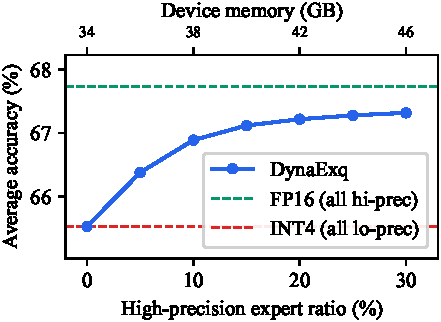
\includegraphics[width=0.48\columnwidth]{figures/budget_sensitivity_qwen30b.pdf}%
  }
  \hfill
  \subfloat[Qwen3-Next-80B]{%
    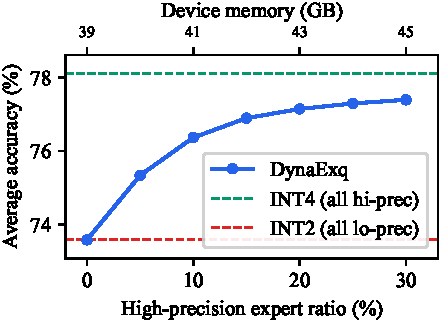
\includegraphics[width=0.48\columnwidth]{figures/budget_sensitivity_qwen80b.pdf}%
  }
  \caption{Average accuracy vs.\ high-precision expert budget ($n_{\mathrm{hi}}/E$). The dashed line marks the static all-low baseline at 0\%.}
  \label{fig:budget_sensitivity}
  \vspace{-1em}
\end{figure}

Both curves exhibit diminishing returns, consistent with a heavy-tailed routing distribution in which a small expert subset receives much of the traffic.

On Qwen3-30B the first 5\% of high-precision experts recovers 0.85\,pp of the 2.20\,pp FP16--INT4 gap, while the next 5\% adds only 0.51\,pp. Each upgrade adds 6.68\,MiB per expert under the packed layout, so the memory price of the first 5\% is already non-trivial. On Qwen3-Next-80B the effect is more pronounced: the first 5\% recovers 1.76\,pp of the 4.54\,pp INT4--INT2 gap, because the wider precision gap amplifies per-expert quality impact while each upgrade adds only 0.703\,MiB. Beyond 25\%, gains on both models fall below 0.1\,pp per 5\% increment. We stop the sweep at 30\% because Qwen3-30B already reaches 46.2\,GB at that point, leaving less than 2\,GB of headroom before the 48\,GB HBM ceiling.

\systemname's default of approximately 20\% lies near the observed knee for both models, recovering 77--79\% of the respective accuracy gap while using 42--43\,GB of the 48\,GB envelope. This shared ratio is descriptive rather than evidence of precision-independent policy optimality. The sweep instead provides a deployment tradeoff: on Qwen3-30B, reducing the ratio from 20\% to 10\% costs approximately 0.33 percentage points while releasing about 4\,GB for other serving state, such as the KV cache.
